\section{Laboratorium nr 4}

\subsection{Interpolacja elementów wektora}\label{lab4/sec/interpolation}
Zdarza się, że posiadamy wektor danych pomiarowych w pewnych chwilach czasu, jednak konieczne jest wyznaczenie wartości dla innej chwili czasu. Np. posiadamy wektor czasu \texttt{[0 0.1 0.2 0.4]} i odpowiadające jemu wartości  \texttt{[2 3 4 6]}, natomiast konieczna jest estymacja wartości dla chwili \texttt{0.3}. Może też istnieć potrzeba zagęszczenia tablicy pomiarów albo obliczenia wartości, która z jakiś powodów jest niewiarygodna bądź niedostępna. 
	
Interpolacja jest metodą numeryczną, która pozwala rozwiązać powyższe problemy. Umożliwia ona estymowanie wartości wektora/funkcji dla niezdefiniowanych argumentów. Funkcją programu MATLAB/GNU Octave, która dokonuje interpolacji jednowymiarowego wektora danych jest \texttt{vq = interp1(x,v,xq)}, gdzie: \texttt{x} jest wektorem czasu (oś X) próbek wejściowych, \texttt{v} jest zbiorem wartości tych próbek (oś Y), natomiast \texttt{xq} jest nowym wektorem czasu dla którego funkcja wyznacza wartości i zwraca wynik w postaci wektora \texttt{vq}. Jako czwarty argument można przekazać rodzaj metody interpolującej. Dostępne są następuje typy interpolacji:
\begin{itemize}
	\item \texttt{'linear'} interpolacja liniowa,
	\item \texttt{'nearest'} interpolacja schodkowa wartością najbliższą,
	\item \texttt{'next'} interpolacja schodkowa wartością następną,
	\item \texttt{'previous'} interpolacja schodkowa wartością poprzednią,
	\item \texttt{'pchip'} interpolacja sklejanymi wielomianami Hermite'a trzeciego rzędu,
	\item \texttt{'spline'} jak wyżej z zaznaczeniem, że interpolujące wielomiany są gładsze.
\end{itemize}


\begin{lstlisting}[caption=Interpolacja danych pomiarowych, label=lab4/lst/interpolationExample]
t = 0:5:50; % input time vector
y = [1 1 10 9 8 7 -5 -5 -10 -10 0]; % values for input vector

t1 = 0:.5:50; % query vector
y1 = interp1(t,y,t1, 'previous');  % zero order hold
y2 = interp1(t,y,t1, 'pchip'); % piecewise cubic interpolation 

% Plot the results
plot(t,y,'o','MarkerSize',12);
hold on;
plot(t1,y1,':^');
plot(t1,y2,':*');
legend('Input vector','next interpolation', 'pchip interpolation');
\end{lstlisting}

\begin{figure}[hbt!]
	\centering
	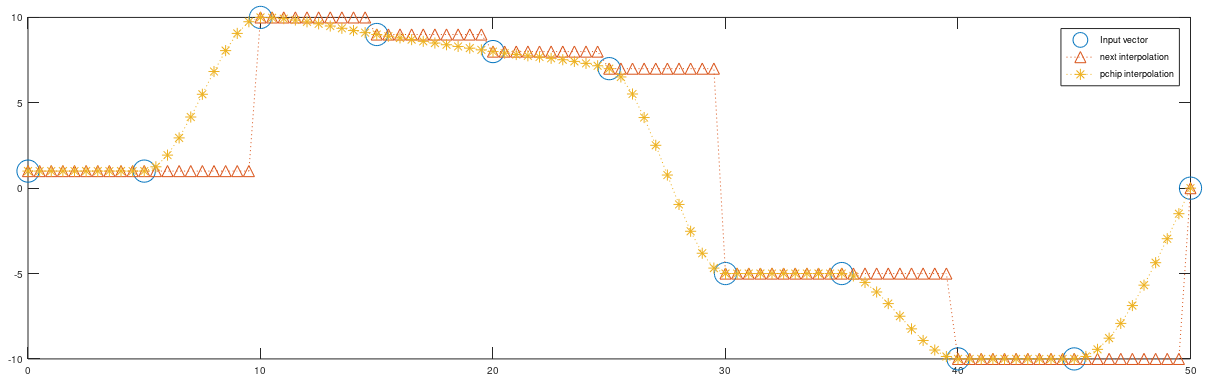
\includegraphics[width=0.95\linewidth]{images/interpolationExample.png}
	\caption{Wykres porównujący dwie metody interpolacji wektora danych wejściowych}
	\label{lab4/fig/interpolationExample}
\end{figure}

Na powyższym listingu~\ref{lab4/lst/interpolationExample} pokazano przykładowe użycie funkcji \texttt{interp1}. Utworzono wejściowy wektor czasu ze skokiem co 5 próbek oraz wektor wartości odpowiadających temu wektorowi czasu. Następnie dodano nowy wektor czasu z krokiem \texttt{0.5}. Posiada on zatem dziesięć razy więcej elementów. Za pomocą funkcji \texttt{interp1} wyznaczono wartości w tych punktach. Nowy wektor posiada zatem dodatkowe próbki z wartościami estymowanymi na podstawie wektora wejściowego.

Na rysunku~\ref{lab4/fig/discriteSignal} pokazano wyniki tej interpolacji. Wejściowy sygnał zaznaczono niebieskimi okręgami. Widać, że tych pomiarów jest niewielka liczba. Następne czerwonymi trójkątami przedstawiono wyniki dla nowego, zagęszczonego wektora czasu, które zostały interpolowane przez podtrzymanie wcześniejszej wartości do momentu pojawienia się nowej próbki (tzw. interpolator zerowego rzędu). Żółtymi gwiazdkami pokazano drugą metodę estymującą wartości za pomocą wielomianów trzeciego rzędu.




\subsection{Próbkowanie i tor przetwarzania sygnałów}
Podczas wcześniejszych zajęć laboratoryjnych sygnały, które były poddawane analizie i przetwarzaniu (np. w postaci filtracji) były ciągłymi sygnałami czasu dyskretnego. Na listingu~\ref{lab4/lst/discreteSignal} pokazano tworzenie wektora danych, tak jak było to robione na poprzednich laboratoriach. Mimo, że funkcja \texttt{plot} standardowo rysuje wykres łącząc kolejne próbki ciągłą linią, dalej są to jedynie wartości funkcji w chwilach wyznaczonych przez wektor czasu~\ref{lab4/fig/discriteSignal}. 

\begin{lstlisting}[caption=Ciągły sygnał czasu dyskretnego, label=lab4/lst/discreteSignal ]
t = 0:.1:2*pi; % time vector
y = sin(t); % value vector
stem(t,y); % stem doesn' connect vector samples using straigh lines
hold on;
plot(t,y); % regular plot which connect samples using straigh lines
\end{lstlisting}

\begin{figure}[hbt!]
	\centering
	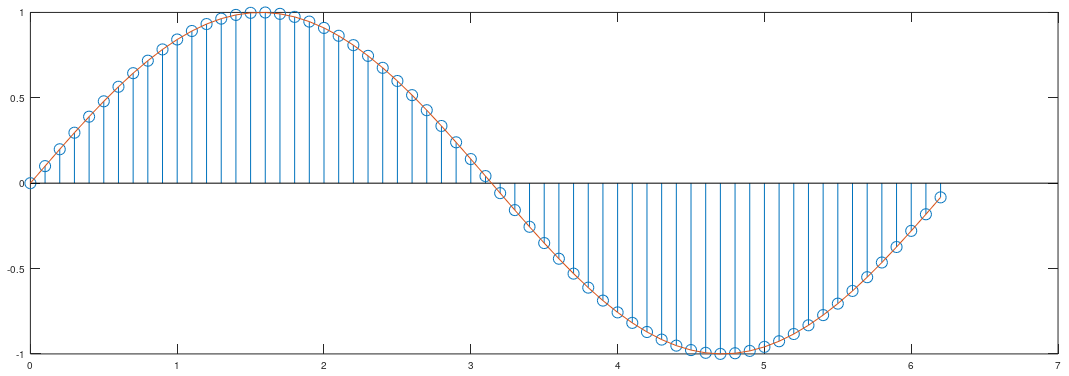
\includegraphics[width=0.95\linewidth]{images/discriteSignal.png}
	\caption{Prezentacja próbek sygnału za pomocą funkcji \texttt{stem} oraz \texttt{plot}}
	\label{lab4/fig/discriteSignal}
\end{figure}

Na rysunku~\ref{lab4/fig/digitalSignalProcessingDiagram} pokazano standardowy tor przetwarzania sygnału analogowego przez układ cyfrowy. W pierwszej kolejności ciągły, analogowy sygnał (np. przebieg napięcia, sygnału audio) jest przy pomocy przetwornika analogowo-cyfrowego przetwarzany na sygnał ciągły czasu dyskretnego tzn. na ciąg próbek sygnału (proces ten nazywany jest \textbf{próbkowaniem}). Takie, już wynikowe, sygnały były tworzone podczas laboratoriów. Dalej sygnał może być analizowany i przetwarzany poznanymi wcześniej metodami. Po tych operacjach możliwe jest ponowne przekształcenie sygnału na postać analogową (ciągłą) przy pomocy przetwornika cyfrowo-analogowego.

\begin{figure}[hbt!]
	\centering
	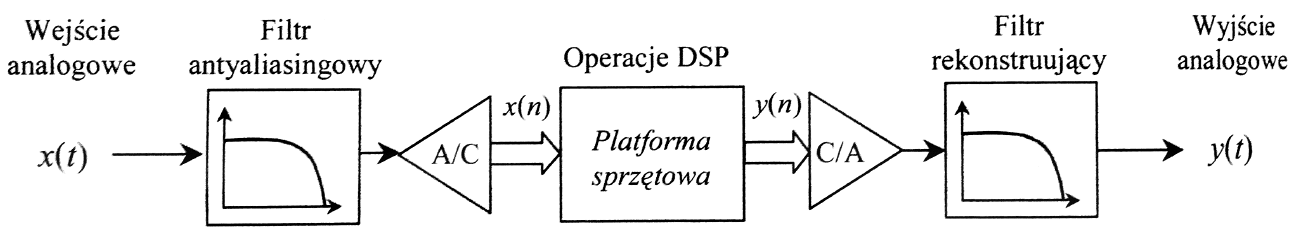
\includegraphics[width=0.9\linewidth]{images/digitalSignalProcessingDiagram.png}
	\caption{Schemat cyfrowego przetwarzania sygnałów~\cite{zielinski_cyfrowe_przetwarzanie_sygnalow}}
	\label{lab4/fig/digitalSignalProcessingDiagram}
\end{figure}

\subsection{Twierdzenie o próbkowaniu}
Twierdzenie o próbkowaniu mówi jaka musi być częstotliwość próbkowania, aby możliwe było późniejsze wierne odtworzenie/zrekonstruowanie próbkowanego sygnału bez zniekształceń. Jest to bardzo istotne twierdzenie zarówno w kontekście przetwarzania sygnałów jak i teorii sterowania. Jak zostało wcześniej wspomniane próbkowanie jest realizowane przez przetwornik analogowo-cyfrowy, który na diagramie został zaznaczony jako A/C~\ref{lab4/fig/digitalSignalProcessingDiagram}.

Najprościej mówiąc twierdzenie to mówi, że funkcja/sygnał nie zawierająca częstotliwościowi większych niż $B$ może być wiernie odtworzona jeżeli częstotliwości próbkowania wynosi $f_s > 2\cdot B$~\ref{lab4/eq/samplingTheorem}. Inaczej mówiąc, jeśli chcemy odtworzyć wszystkie częstotliwości w sygnale, musimy go próbkować z dwa razy większą częstotliwością niż częstotliwość najwyższej składowej. Jest to powód dlaczego sygnały audio są kodowane z częstotliwością $48~kHz$ (jakość DVD). Ludzki słuch posiada zakres słyszalnych częstotliwości w zakresie od $16$ do $20000~Hz$. Aby móc odtworzyć maksymalną częstotliwość jaką człowiek jest w stanie usłyszeć należy próbkować z częstotliwością dwa razy większą niż najwyższa składowa, w tym przypadku $20~kHz$.

\begin{equation}\label{lab4/eq/samplingTheorem}
	B < \frac{f_s}{2}
\end{equation}

Załóżmy, że nasz sygnał zawiera jedną składową o danej częstotliwości. Potrzeba minimum dwóch pomiarów pomiędzy pojedynczym okresem, aby odtworzyć tę składową. Jeśli będziemy próbkować rzadziej to inna funkcja o niższej częstotliwości będzie mogła interpolować te punkty. Takie niepożądane zjawisko nazywane jest aliasingiem. Aliasing sprawia, że tracimy w sygnale informacje o składowych, które mogą nas interesować.

Na rysunku~\ref{lab4/fig/aliasedComponent} pokazano widmo sygnału sinusoidalnego o częstotliwości $700~Hz$, który został spróbkowany z częstotliwością równą $1000~Hz$, warunki twierdzenia o próbkowaniu w tym przypadku nie zostały zachowane. Składowa sygnału jest wyższa niż połowa częstotliwości próbkowania, która nazywana jest częstotliwością Nyquista ($f_N = \frac{f_s}{2} = 500~Hz$). W wyniku zjawiska aliasingu została ona odbita/,,zawinięta'' względem $f_N$. Przy próbie rekonstrukcji tego sygnału np. przez przetwornik cyfrowo-analogowy zaobserwowana częstotliwość będzie wynosić $300~Hz$.

\begin{figure}[hbt!]
	\centering
	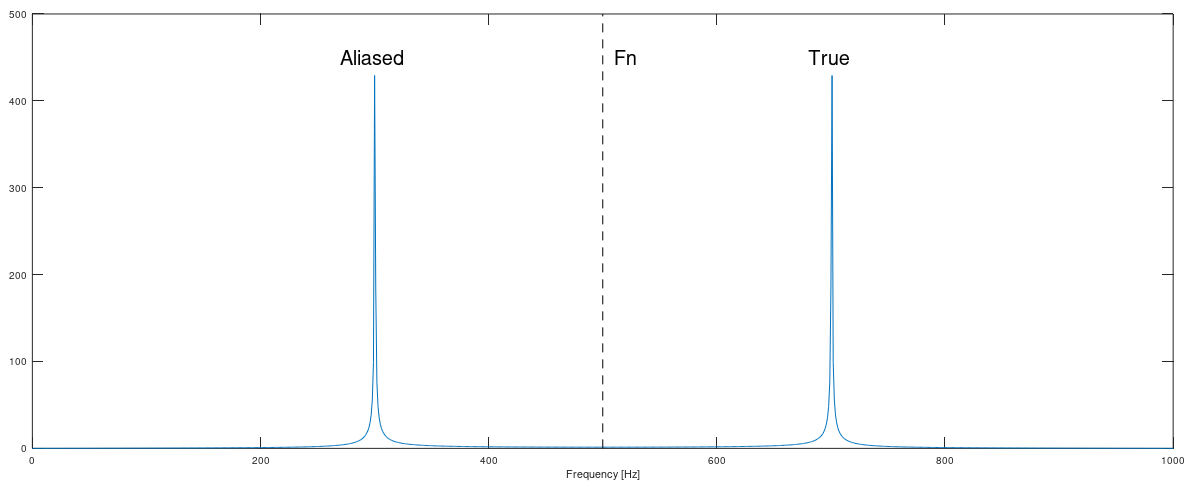
\includegraphics[width=0.95\linewidth]{images/aliasedComponent.png}
	\caption{Widmo sygnału sinusoidalnego o częstotliwości $700~Hz$ próbkowanego z częstotliwością $1000~Hz$.}
	\label{lab4/fig/aliasedComponent}
\end{figure}

Na listingu~\ref{lab4/lst/recostructionOfDownsamplesSignal} zademonstrowano w programie MATLAB/GNU Octave zmianę częstotliwości próbkowania. Najpierw stworzono wektor danych sygnału sinusoidalnego o częstotliwości $100~Hz$ próbkowanego z częstotliwością $1000~Hz$, zgodnie z twierdzeniem o próbkowaniu możliwe jest jego wierne odtworzenie w postać analogową. Następnie dodano nowy wektor czasu tym razem z odstępami pomiędzy próbkami $\frac{1}{110}$, czyli w tym przypadku częstotliwość próbkowania wyniosła $110~Hz$. Dalej wyznaczono wektor wartości funkcji sinusoidalnej o częstotliwości $100~Hz$ tak jak poprzednio z tą różnicą, że tym razem dla nowego wektora czasu ze znacznie mniejszą liczbą argumentów. Na koniec podjęto próbę interpolacji (rekonstrukcji) sygnału tak, aby ponownie uzyskać próbki pomiędzy węzłami (próbkami) drugiego z sygnałów. Inaczej mówiąc chcieliśmy na podstawie wektora z mniejszą liczbą próbek wyznaczyć wartości sygnału w chwilach zdefiniowanych przez pierwszy wektor czasu (z próbkami rozmieszczonymi co $\frac{1}{1000}$).
\begin{lstlisting}[caption=Symulacja niedostatecznie wysokiej częstotliwości próbkowania, label=lab4/lst/recostructionOfDownsamplesSignal]
Fs = 1000;
t1=0:1/Fs:1;
y1=sin(2*pi*100*t1); % sinusoidal signal with 100 Hz frequency

Fs2 = 110;
t2=0:1/Fs2:1; % simulation of sampling with frequency of 100 Hz
y2 = sin(2*pi*100*t2);
vq2 = interp1(t2,y2,t1,'spline');

subplot(211);
plot(t1,y1); title('Original signal'); % original signal
subplot(212)
plot(t1,vq2); title('Output signal reconstructed from downsampled original'); % output signal reconstructed from downsampled original
\end{lstlisting}

Poniżej~\ref{lab4/fig/downsampledSignal} pokazano przebiegi wynikowe omawianego wyżej kodu źródłowego. Widać, że przez niedostateczne próbkowanie po rekonstrukcji sygnał wejściowy ma zdecydowanie niższą częstotliwość, został zniekształcony przez proces konwersji i zbyt niską częstotliwość próbkowania. Analizując sygnał w dziedzinie częstotliwości należałoby oczekiwać prążka dla argumentu $100~Hz$. W związku, że częstotliwość próbkowania została obniżona do $110~Hz$, ,,prążek'' na widmie sygnału znalazł się po prawej stronie częstotliwości Nyquista i został odbity symetrycznie względem niej. W wyniku czego ,,prążek'' pojawił się w częstotliwości $10~Hz$, której pierwotnie nie było w sygnale.

\begin{figure}[hbt!]
	\centering
	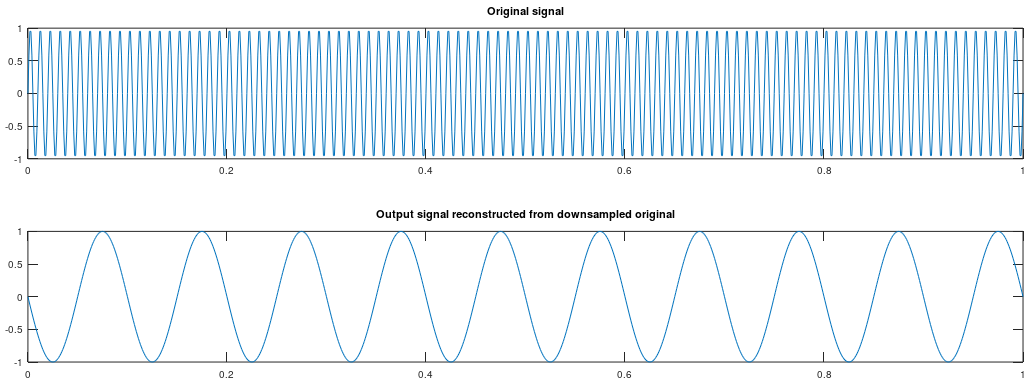
\includegraphics[width=0.95\linewidth]{images/downsampledSignal.png}
	\caption{Oryginalny sygnał o częstotliwości $100~Hz$ po próbkowaniu z niedostateczną częstotliwością po rekonstrukcji został zniekształcony.}
	\label{lab4/fig/downsampledSignal}
\end{figure}


Efekt aliasingu można zaobserwować również na nagraniach z kamery wideo, jeśli nagrywana osoba posiada jakiś wzór na obraniach (szachownicę, siatkę, drobne prążki) to kamera może powodować efekt aliasingu podczas poruszania się tej osoby (efekt błyszczenia). To zjawisko można również zauważyć na poniższym zdjęciu~\ref{lab4/fig/zonePlate}. Przy zmniejszeniu rozmiaru strony w pliku PDF np. przez użycie kółka myszy z wciśniętym przyciskiem CTRL, widać pojawiające się artefakty.
\begin{figure}[hbt!]
	\centering
	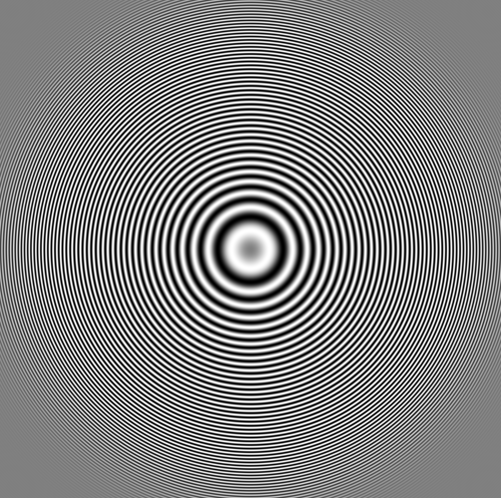
\includegraphics[width=0.5\linewidth]{images/zonePlate.png}
	\caption{Przykładowe zdjęcie na którym można zaobserwować zjawisko aliasingu.}
	\label{lab4/fig/zonePlate}
\end{figure}



\subsection{Zadania}
\subsubsection{Interpolacja wektora danych pomiarowych}
Na listingu~\ref{lab4/lst/interpolationExample} pokazano przykład interpolacji danych pomiarowych za pomocą dwóch metod: interpolatorem zerowego rzędu (ang. Zero Order Hold) oraz sklejanymi wielomianami Hermite'a trzeciego rzędu. Przetestuj wszystkie wymienione w podpunkcie~\ref{lab4/sec/interpolation} metody wywołując funkcję \texttt{interp1} ze zmienionym czwartym argumentem, w którym przekazywana jest metoda interpolacji.
\subsubsection{Widmo sygnału dla różnych częstotliwości próbkowania}
Utwórz sygnał sinusoidalny o częstotliwości $500~Hz$. Wyznacz wartości tego przebiegu dla co najmniej jeden sekundy, przyjmując częstotliwość próbkowania równą $2000~Hz$.
\begin{lstlisting}[caption=Symulacja niedostatecznie wysokiej częstotliwości próbkowania, label=lab4/lst/recostructionOfDownsamplesSignal]
Fs = 2000;
t1=0:1/Fs:1;
y1=sin(2*pi*500*t1); % sinusoidal signal with 100 Hz frequency
\end{lstlisting}
Wyznacz widmo tego sygnału w zakresie częstotliwości $f\in[0;\frac{f_s}{2}]$ tak jak robiliśmy to na drugich laboratoriach~\ref{lab2/lst/fftExample}. Powinieneś zaobserwować pojedynczy prążek dla częstotliwości $500~Hz$.

Teraz powtórz ten sam proces zmieniając częstotliwość próbkowania odpowiednio $f_s \in \{1100; 900; 700; 600\}$. Zaobserwuj moment przekraczania granicy Nyquista i zawinięcia się widma, wyższe częstotliwości przechodzącą na stronę pasma poniżej połowy częstotliwości próbkowania.


\subsubsection{Rekonstrukcja sygnału ze zbyt niskim okresem pomiędzy próbkami}
Podobnie jak w przykładzie~\ref{lab4/lst/recostructionOfDownsamplesSignal} spróbuj interpolować sygnał utworzony w poprzednim zadaniu z częstotliwością próbkowania równą $600~Hz$. Utwórz nowy wektor czasu tak, aby interpolowany sygnał miał częstotliwość próbkowania ponownie $2000~Hz$ np. w następujący sposób: \texttt{t = 0:1/2000:1}. Wykorzystując funkcję \texttt{interp1} wyznacz nowy wektor wartości dla nowego wektora czasu. Narysuj otrzymany sygnał. Zwróć uwagę, że tak jak pokazywała analiza częstotliwościowa nie udało się zrekonstruować częstotliwości $500~Hz$. W procesie rekonstrukcji została ona ,,zawinięta'' i stała się składową o częstotliwości $100~Hz$.